\documentclass{article}

%\usepackage[paperwidth=8in, paperheight=11.5in]{geometry}
\usepackage[
    paperwidth=1.89in,
    paperheight=19in,
    margin=0.2in,
]{geometry}

\usepackage{pifont}
\usepackage{utfsym}

\usepackage{tikz}
\usetikzlibrary{shapes,backgrounds}




\newcommand{\sep}{\vskip7ex}

\pagenumbering{gobble}

% SEE https://tex.stackexchange.com/questions/58903/how-to-draw-star-in-tikz-background
\newcommand{\tstar}[5]{% inner radius, outer radius, tips, rot angle, options
\pgfmathsetmacro{\starangle}{360/#3}
\draw[#5] (#4:#1)
\foreach \x in {1,...,#3}
{ -- (#4+\x*\starangle-\starangle/2:#2) -- (#4+\x*\starangle:#1)
}
-- cycle;
}


% two 8 point stars, the second smaller and rotated 45
\newcommand{\dstar}[5]{% inner radius, outer radius, rot angle, options, innerscale
\pgfmathsetmacro{\starangle}{360/4}
\begin{scope}
\draw[#4] (#3:#1)
\foreach \x in {1,...,4}
{ -- (#3+\x*\starangle-\starangle/2:#2) -- (#3+\x*\starangle:#1)}
-- cycle;
\end{scope}
\begin{scope}[rotate=\starangle/2, scale=#5]
\draw[#4] (#3:#1)
\foreach \x in {1,...,4}
{ -- (#3+\x*\starangle-\starangle/2:#2) -- (#3+\x*\starangle:#1)}
-- cycle;
\end{scope}
}


\newcommand{\ngram}[4]{% outer radius, tips, rot angle, options
\pgfmathsetmacro{\starangle}{360/#2}
\pgfmathsetmacro{\innerradius}{#1*sin(90-\starangle)/sin(90+\starangle/2)}
\tstar{\innerradius}{#1}{#2}{#3}{#4}
}

\begin{document}


%\usym{2726}  % 4
%\usym{2605}  % 5
%\usym{2736}  % 6
%\usym{2734}  % 8
%\usym{2737}  % 8
%\usym{2739}  % 12
%\usym{2728}  % three parabola
%\usym{263D}  % moon
%\usym{1F31E} % sun

\begin{centering}

% 5 star
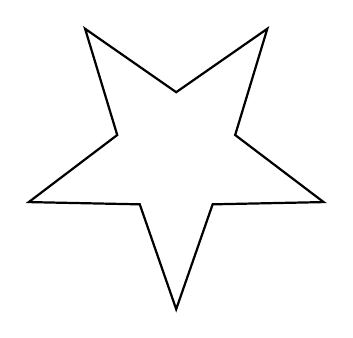
\begin{tikzpicture}[scale=0.3937] %  0.3937 is approximately the conversion factor from cm to inches (1 cm = 0.3937 in)
    \tstar{2}{5}{5}{18}{thick}
\end{tikzpicture}
\sep

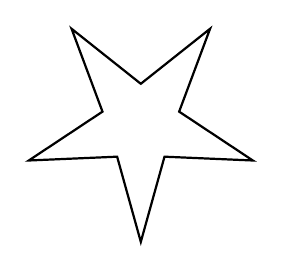
\begin{tikzpicture}[scale=0.3937] %  0.3937 is approximately the conversion factor from cm to inches (1 cm = 0.3937 in)
    \tstar{1.3}{3.8}{5}{18}{thick}
\end{tikzpicture}
\sep

% 6 star
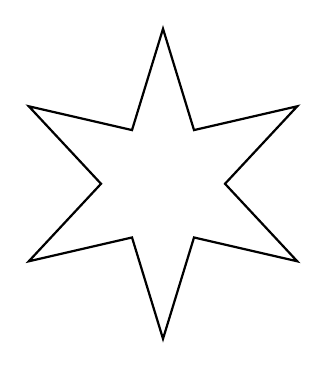
\begin{tikzpicture}[scale=0.3937] %  0.3937 is approximately the conversion factor from cm to inches (1 cm = 0.3937 in)
    \tstar{2}{5}{6}{0}{thick}
\end{tikzpicture}
\sep

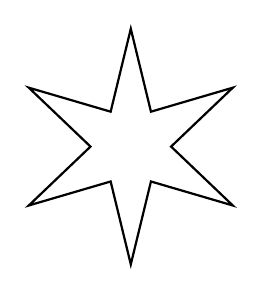
\begin{tikzpicture}[scale=0.3937] %  0.3937 is approximately the conversion factor from cm to inches (1 cm = 0.3937 in)
    \tstar{1.3}{3.8}{6}{0}{thick}
\end{tikzpicture}
\sep

% 7 star

\begin{tikzpicture}[scale=0.3937] %  0.3937 is approximately the conversion factor from cm to inches (1 cm = 0.3937 in)
    \tstar{2}{5}{7}{12.8}{thick}
\end{tikzpicture}
\sep


\begin{tikzpicture}[scale=0.3937] %  0.3937 is approximately the conversion factor from cm to inches (1 cm = 0.3937 in)
    \tstar{1.3}{3.8}{7}{12.8}{thick}
\end{tikzpicture}
\sep

% 8 star
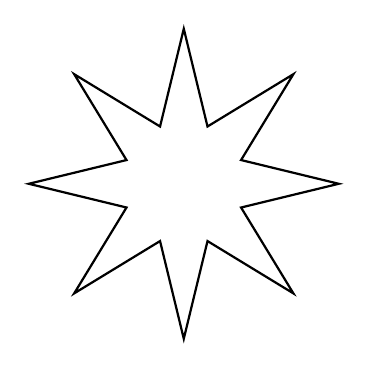
\begin{tikzpicture}[scale=0.3937] %  0.3937 is approximately the conversion factor from cm to inches (1 cm = 0.3937 in)
    \tstar{2}{5}{8}{22.5}{thick}
\end{tikzpicture}
\sep

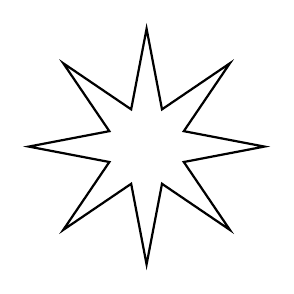
\begin{tikzpicture}[scale=0.3937] %  0.3937 is approximately the conversion factor from cm to inches (1 cm = 0.3937 in)
    \tstar{1.3}{3.8}{8}{22.5}{thick}
\end{tikzpicture}
\sep


% double star
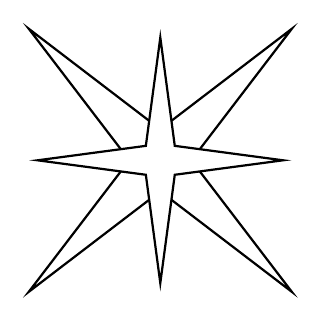
\begin{tikzpicture}[scale=0.3937] %  0.3937 is approximately the conversion factor from cm to inches (1 cm = 0.3937 in)
    \dstar{1}{6}{0}{thick,fill=white}{0.66}
\end{tikzpicture}
\sep

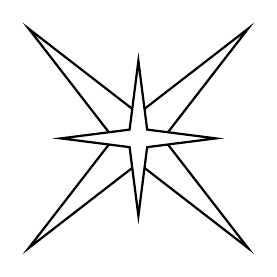
\begin{tikzpicture}[scale=0.3937] %  0.3937 is approximately the conversion factor from cm to inches (1 cm = 0.3937 in)
    \dstar{0.8}{5}{0}{thick,fill=white}{0.5}
\end{tikzpicture}
\sep

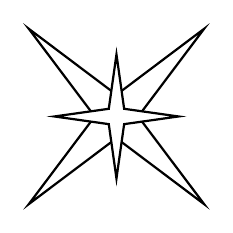
\begin{tikzpicture}[scale=0.3937] %  0.3937 is approximately the conversion factor from cm to inches (1 cm = 0.3937 in)
    \dstar{0.7}{4}{0}{thick,fill=white}{0.5}
\end{tikzpicture}
\sep



\end{centering}
\end{document}
